\documentclass[blue]{beamer}
%\documentclass[handout]{beamer}

%\beamerboxesdeclarecolorscheme{alert}{brown}{brown!25!averagebackgroundcolor}

\usepackage{beamerthemeshadow}
\usepackage[ngerman]{babel}
\usepackage[ansinew]{inputenc}
\usepackage{html,makeidx}
%\usecolortheme{whale}


%%%%%%%%%%%%%%%%%%%%%%%%%%%%%%%%%%%%%%%%%%%%%%%%%%%%%%%%%%%%%%%%%%%%%%%%%%%%%%%%%%%%
%%%%%%%%%%%%%%%%%%%%%%%%%%%%%%%%%%%%%%%%%%%%%%%%%%%%%%%%%%%%%%%%%%%%%%%%%%%%%%%%%%%%

\title{METANET - Interactive Knowledge Network}
\institute[META-D.O.N]{META-D.O.N\\Association for Cultural Substitution Services}
\author{Hannes Weingartner}
\date{April 17, 2010}

\begin{document}
\frame{\titlepage}

% no entry in TOC but in the navigation bar
\section*{overview}
\frame{\tableofcontents}


%%%%%%%%%%%%%%%%%%%%%%%%%%%%%%%%%%%%%%%%%%%%%%%%%%%%%%%%%%%%%%%%%%%%%%%%%%%%%%%%%%%%
%%%%%%%%%%%%%%%%%%%%%%%%%%%%%%%%%%%%%%%%%%%%%%%%%%%%%%%%%%%%%%%%%%%%%%%%%%%%%%%%%%%%


\section{project}
\subsection{introduction}
\frame
{
\frametitle{\textbf{introduction}}
\begin{itemize}
\item the technical part of a project of the\textbf{ meta-d.o.n association}: sociocultural studies in serbia called \textbf{New[B]Order} - \htmladdnormallink{http://www.meta-don.org/newborder/}{http://www.meta-don.org/newborder/}
\item concept of a spatial \textbf{knowledge network}
\item web-based application for linking \textbf{spatial and sematic data}
\item based on \textbf{free- and open source software components}
\end{itemize}
}

\subsection{goal}
\frame
{
\frametitle{\textbf{goal}}
\begin{itemize}
\item \textbf{flexiblity in usage:} generic tool for scientific research projects
\item \textbf{administration:} intuitive CMS interface for researchers
\item \textbf{METABLOG - artifacts input:}
  \begin{itemize}
    \item text, sound, images, an mm data through CMS
    \item mobile devices for geo-tagged content input
  \end{itemize}
\item \textbf{METAMAP: 2D map for customized geo-spatial representation of artifacts}
\item \textbf{METASPACE: 3D semantic graph/subgraph associated with map artifacts}
\item algorithms for finding similarities/references between artifacts
\item \textbf{usability:} advanced hardware and software interfaces to the user (e.g for exhibitions)
\item \textbf{statistics}
\end{itemize}
}

\frame
{
\frametitle{\textbf{domains}}
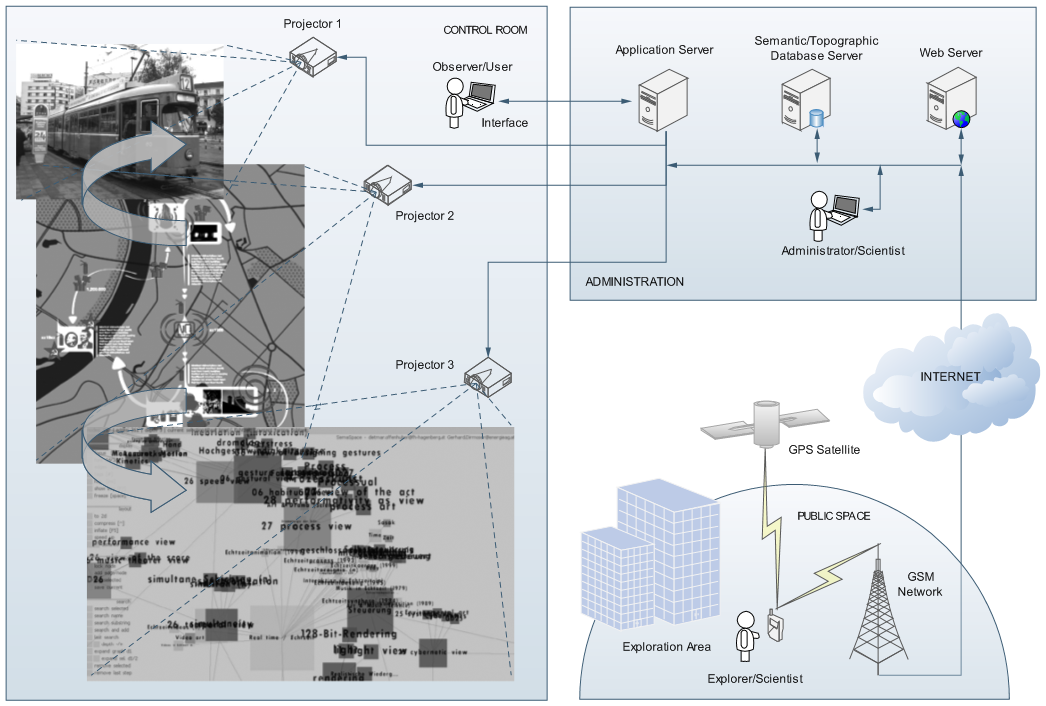
\includegraphics[width=0.95\textwidth]{bin/domains/domains.png}
}


\subsection{challenges}
\frame
{
\frametitle{\textbf{challenges}}
\begin{itemize}
\item \textbf{customization of map} for adequate content representation
\item \textbf{administration:} intuitive CMS interface for researchers
\item \textbf{data consistency} between METAMAP and METASPACE
\item \textbf{METASPACE hardware HCI} design and implementation
\end{itemize}
}


\subsection{technologies}
\frame
{
\frametitle{\textbf{technologies}}
\begin{itemize}
\item \textbf{language:} java and java script
\item \textbf{dependencies:}
  \begin{itemize}
    \item \textbf{Semaspace} (http://residence.aec.at/didi/FLweb/)
    \item \textbf{OpenStreetMap} aka OSM (http://www.openstreetmap.org/)
    \item \textbf{Google Web Toolkit 2.0} aka GWT (http://code.google.com/webtoolkit/)
  \end{itemize}
\end{itemize}
}

%%%%%%%%%%%%%%%%%%%%%%%%%%%%%%%%%%%%%%%%%%%%%%%%%%%%%%%%%%%%%%%%%%%%%%%%%%%%%%%%%%%%
%%%%%%%%%%%%%%%%%%%%%%%%%%%%%%%%%%%%%%%%%%%%%%%%%%%%%%%%%%%%%%%%%%%%%%%%%%%%%%%%%%%%

% TODO research:  knowledge network

% TODO research: virtools technical + developers
\section{semaspace}
\subsection{outline}
\frame
{
\frametitle{\textbf{outline}}
\begin{itemize}
	\item \textbf{fast opengl accelerated graph editor and browser} for large knowledge networks
	\item developed by \textbf{dietmar offenhuber and gerhard dirmoser - fh hagenberg}
	\item \textbf{interactive graph layout} in 2d and 3d
	\item \textbf{nodes} can incorporate data such as images, sound and text
	\item \textbf{java swt} desktop application
	\item embedding into web clients with \textbf{virtools webplayer}
	\item the network is represented by so called edge files
	\item presentent at the \textbf{ars electronica festival 2003}
	\item ui for \textbf{web clients} and \textbf{exhibitions}
\end{itemize}
}

\subsection{dependencies}
\frame
{
\frametitle{\textbf{dependencies}}
\begin{itemize}
	\item \textbf{jogl:} open source java binding to opengl api from sun (for harware supported 3d graphics)
	\item \textbf{jftgl:} java based lib for accessing tt fonts within opengl
	\item \textbf{apache batik svg toolkit:} open source java based toolkit for using images in the svg format (xml based)
	\item \textbf{\htmladdnormallink{semaspace demo}{file:///C:/Users/hn/Workspace-Java/metanet/files/presentation/bin/semaspace/web-demo/semaspace.html}}
\end{itemize}
}


\subsection{extensions}
\frame
{
\frametitle{\textbf{extensions}}
\begin{itemize}
	\item \textbf{video nodes}
	\item \textbf{remote graph access and manipulation} through network connections
	\item research and implementation of \textbf{extending hardware interfaces} for browsing
		\begin{itemize}[<+-|alert@+>]
			\item browsing (zoom, rotation)
			\item 2d/3d
			\item fog
			\item freeze
			\item node distance
		\end{itemize}
\end{itemize}
}


%%%%%%%%%%%%%%%%%%%%%%%%%%%%%%%%%%%%%%%%%%%%%%%%%%%%%%%%%%%%%%%%%%%%%%%%%%%%%%%%%%%%
%%%%%%%%%%%%%%%%%%%%%%%%%%%%%%%%%%%%%%%%%%%%%%%%%%%%%%%%%%%%%%%%%%%%%%%%%%%%%%%%%%%%













%%%%%%%%%%%%%%%%%%%%%%%%%%%%%%%%%%%%%%%%%%%%%%%%%%%%%%%%%%%%%%%%%%%%%%%%%%%%%%%%%%%%
%%%%%%%%%%%%%%%%%%%%%%%%%%%%%%%%%%%%%%%%%%%%%%%%%%%%%%%%%%%%%%%%%%%%%%%%%%%%%%%%%%%%


\section*{Summary}
\frame
{
\frametitle{\textbf{Summary}}
\begin{itemize}
\item \textbf{METANET - Interactive Knowledge Network}
\end{itemize}
}

%%%%%%%%%%%%%%%%%%%%%%%%%%%%%%%%%%%%%%%%%%%%%%%%%%%%%%%%%%%%%%%%%%%%%%%%%%%%%%%%%%%%

\frame[plain]
{
\begin{center}
{\Large\textbf{Thank You.}}
\end{center}
}

\end{document}

%%%%%%%%%%%%%%%%%%%%%%%%%%%%%%%%%%%%%%%%%%%%%%%%%%%%%%%%%%%%%%%%%%%%%%%%%%%%%%%%%%%%


%\begin{beamerboxesrounded}[scheme=alert,shadow=true]{simple.xul}
%\end{beamerboxesrounded}
%\hyperlink{packages<2>}{\beamergotobutton{packages item 2}}


%\frame
%{
%\frametitle{\textbf{title}}
%\begin{itemize}
%\item<1-|alert@1>\textbf{item}
%	\begin{itemize}
%		\item<3-|alert@3> item
%	\end{itemize}
%\item<2-|alert@2>\textbf{item}
%	\begin{itemize}
%		\item<4-|alert@4> item
%	\end{itemize}
%\end{itemize}
%}




